
\providecommand{\rvF}{\mathbf{F}}  %
\providecommand{\rvW}{\mathbf{W}}  %
\providecommand{\rvWarrow}{\rightsquigarrow}%
\providecommand{\rvFarrow}{\twoheadrightarrow}%
\providecommand{\rvTFarrow}{\rightsquigarrow\joinrel\twoheadrightarrow}%

\section{纤维性对象范畴中的抽象同伦论}\label{sec:abstract-homotopy-theory-in-a-category-of-fibrant-objects}

在本节中，我们在一个（非富集的）\textbf{\trCategoryOfFibrantObjects}（category of fibrant
objects）中工作；这一概念由 Brown \cite{bib23} 首次引入。例子包括一个%
\trInfinityCosmos{}的底范畴，或一个 Quillen \trModelCategory{}中\trFibrant{}对象的
全子范畴（full subcategory）——「\trCategoryOfFibrantObjects」之名即由此而来。

\begin{definition}[\trCategoryOfFibrantObjects]\label{def:category-of-fibrant-objects}
一个\textbf{\trCategoryOfFibrantObjects}由一个\trCategory{} $\mathcal{M}$ 连同态射的两个%
子范畴 $\rvW$ 与 $\rvF$ 构成，并满足如下公理：
\begin{enumerate}[label=(\roman*)]
\item $\mathcal{M}$ 拥有\trProduct{}，特别地拥有一个\trTerminal{}对象 $1$。
  而且，类 $\rvF$ 与 $\rvF\cap\rvW$ 各自对\trProduct{}封闭。
\item $\rvW$ 具有\textbf{\trTwoOfThreeProperty}：对任何可复合的一对态射，
  若 $f$、$g$ 与 $gf$ 三者中的任两个属于 $\rvW$，则第三个亦然。
\item $\rvF$ 中诸映射的\trPullback{}存在且仍落于 $\rvF$ 中，且类
  $\rvF\cap\rvW$ 在\trPullback{}下亦稳定。
\item $\rvF$ 中诸映射的可数塔\footnote{一个（可数）\textbf{塔}（tower）是
  形状为 $\omega^{\mathrm{op}}$ 的图表。对塔的\trLimit{}封闭断言：若塔中每支
  原子箭头的像均落于 $\rvF$ 中，则从图表中的\trLimit{}对象到其中%
  \trTerminal{}对象的映射亦在 $\rvF$ 中。对偶概念——从 $\omega$ 形图表中%
  \trInitial{}对象到其\trColimit{}的映射——通常称作「可数复合」
  （countable composite），在更大的极限序数情形下则称「超限复合」
  （transfinite composite）。以其他极限序数为标的更一般的塔，在%
  \cref{lem:right-lifting-closure}及其后考虑。}的\trLimit{}存在且也落于 $\rvF$ 中，且类 $\rvF\cap\rvW$
  对塔之\trLimit{}的构造同样封闭。
\item 对每个对象 $B$，都存在一个\textbf{\trPathObject} $PB$，连同对角的%
  一个因子分解——先是一支属于 $\rvW$ 的映射，继之一支属于 $\rvF$ 的映射：
  \begin{center}
  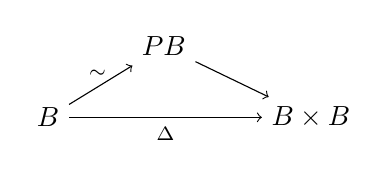
\begin{tikzpicture}[x=1.9em,y=1.35em]
    \node (pb) at (2.2,1.9) {$PB$};
    \node (b) at (0,0) {$B$};
    \node (bb) at (5.0,0) {$B\times B$};
    \draw[->] (b) -- node[above,pos=0.45]{$\scriptstyle\sim$} (pb);
    \draw[->] (pb) -- (bb);
    \draw[->] (b) -- node[below]{$\scriptstyle\Delta$} (bb);
  \end{tikzpicture}
  \end{center}
\item 一切对象都是\textbf{\trFibrant}{}的：对每个 $B\in\mathcal{M}$，映射
  $B\to 1$ 落于 $\rvF$ 中。
\end{enumerate}
\end{definition}

\begin{remark}\label{rem:original-definition}
原始定义在公理 (i) 中只要求有限\trProduct{}的存在性，并且省去了公理 (iv)。
类 $\rvF$ 与 $\rvF\cap\rvW$ 对有限\trProduct{}的封闭性，可由公理 (iii) 所
假设的对\trPullback{}的封闭性经归纳推得（见\cref{cor:finite-products}）。
在此，我们提出这些无穷\trLimit{}的要求，以与我们∞-\trInfinityCosmos{}定义中的%
\trLimit{}公理——第 1 章中的\cref{def:infinity-cosmos}(i)——相平行。实践中，
类 $\rvF$ 与 $\rvF\cap\rvW$ 常由一个右提升性质（right lifting property）
来刻画，此时封闭公理 (i)、(iii) 与 (iv) 自动成立（见\cref{lem:right-lifting-closure}）。
\end{remark}

一般而言，习惯上把 $\rvW$ 中的映射称作「\trWeakEquivalence」，把 $\rvF$ 中的
映射称作「\trFibration」，而把 $\rvF\cap\rvW$ 中的映射称作「\trTrivialFibration」
——除非具体语境要求别样的名称——并分别用装饰箭头
$\rvWarrow$、$\rvFarrow$ 与 $\rvTFarrow$ 来描绘这三个类。我们之所以对%
\trCategoryOfFibrantObjects{}怀有首要的兴趣，正是缘于以下两个例子。

\begin{example}\label{exa:cosmos-as-fibrant-objects}
一个\trInfinityCosmos{}的底范畴定义了一个\trCategoryOfFibrantObjects，其中取 $\rvW$ 为%
\trEquivalence{}类，$\rvF$ 为\trIsofibration{}类。\cref{def:category-of-fibrant-objects}
的多数公理已被第 1 章中的\cref{def:infinity-cosmos} 的\trLimit{}公理与%
\trIsofibration{}公理所涵盖；余下的部分则在\cref{lem:trivial-fibration-stability}、%
\cref{lem:equivalence-retracts-2-of-3} 与\cref{lem:brown-factorization}中建立。
\end{example}

\begin{example}\label{exa:model-category-fibrant-objects}
一个\trModelCategory{}中\trFibrant{}对象的全子范畴定义了一个\trCategoryOfFibrantObjects，
其中取 $\rvW$ 为\trWeakEquivalence{}类，$\rvF$ 为\trFibrant{}对象之间的%
\trFibration{}类（见\cref{def:fibrant-cofibrant} 与\cref{ex:fibrant-objects-from-model}）。
\end{example}

\begin{remark}\label{rem:right-proper}
刚刚讨论的两个例子都具有\textbf{\trRightProper}这一附加性质，即满足下面的%
一条附加公理：

(vii) $\rvW$ 中的映射沿 $\rvF$ 中映射的\trPullback{}仍是 $\rvW$ 中的映射：
\begin{center}
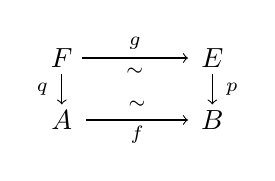
\begin{tikzpicture}[x=1.6em,y=1.6em]
  \node (tl) at (0,1.4) {$F$};
  \node (tr) at (3.4,1.4) {$E$};
  \node (bl) at (0,0) {$A$};
  \node (br) at (3.4,0) {$B$};
  \draw[->] (0.45,1.4) -- (2.85,1.4);
  \node at (1.65,1.74) {$\scriptstyle g$};
  \node at (1.65,1.1) {$\scriptstyle\sim$};
  \draw[->] (0,1.05) -- (0,0.35);
  \node at (-0.44,0.7) {$\scriptstyle q$};
  \node at (0.48,0.78) {$\scriptstyle\lrcorner$};
  \draw[->] (3.4,1.05) -- (3.4,0.35);
  \node at (3.84,0.7) {$\scriptstyle p$};
  \draw[->] (0.55,0) -- (2.85,0);
  \node at (1.7,-0.34) {$\scriptstyle f$};
  \node at (1.7,0.34) {$\scriptstyle\sim$};
\end{tikzpicture}
\end{center}
\end{remark}

对∞-宇宙而言，这在第 3 章中的\cref{prop:pullback-equivalence} 中得到证明；
而对模型范畴中的纤维性对象，这首先由 Reedy 在 \cite[Theorem B]{bib99} 中
观察到（另见 \cite[15.4.2]{bib84}）。

\trCategoryOfFibrantObjects{}中的分解公理可以推广，以构造任意映射的分解
（见第 1 章中的\cref{lem:brown-factorization}）。

\begin{lemma}[Brown 分解引理]\label{lem:brown-factorization-cfo}
\trCategoryOfFibrantObjects{}中的任何映射 $f\colon A\to B$ 都可以分解为一支%
\trWeakEquivalence{}继以一支\trFibration，其中该\trWeakEquivalence{}被%
构造为一支\trTrivialFibration{}的\trSection。
\begin{center}
\begin{tikzpicture}[x=1.6em,y=1.6em]
  \node (Pf) at (0.6,1.5) {$Pf$};
  \node (A) at (-1.4,0) {$A$};
  \node (B) at (3.0,0) {$B$};
  \draw[double,->] (Pf) to[bend right=28] node[pos=0.55,above,sloped]{$\scriptstyle\overset{\sim}{q}$} (A);
  \draw[->] (A) to[bend right=22] node[pos=0.5,below,sloped]{$\scriptstyle s$} (Pf);
  \draw[double,->] (Pf) -- node[pos=0.45,above,sloped]{$\scriptstyle p$} (B);
  \draw[->] (A) -- node[below]{$\scriptstyle f$} (B);
\end{tikzpicture}
\end{center}
此外，$f$ 是\trWeakEquivalence{}当且仅当\trFibration{} $p$ 是%
\trTrivialFibration。
\end{lemma}

\begin{proof}
图中所示的分解由 (v) 中\trPathObject{}分解 $B\rvWarrow PB\rvFarrow B\times B$
的\trPullback{}构造：
\begin{center}
\begin{tikzpicture}[x=1.6em,y=1.5em]
  \node (A) at (0,2.3) {$A$};
  \node (B) at (2.6,2.3) {$B$};
  \node (Pf) at (1.0,1.1) {$Pf$};
  \node (PB) at (2.9,1.1) {$PB$};
  \node (AB) at (0,0) {$A\times B$};
  \node (BB) at (3.5,0) {$B\times B$};
  \draw[->] (0.45,2.3) -- (2.1,2.3) node[midway,above]{$\scriptstyle f$};
  \draw[dashed,->] (0.1,2.0) -- (0.75,1.4) node[pos=0.4,left]{$\scriptstyle\overset{\sim}{s}$};
  \draw[->] (A) to[out=-105,in=115] node[pos=0.5,left]{$\scriptstyle(A,f)$} (AB);
  \draw[->] (0.8,0.85) -- (0.2,0.25) node[pos=0.45,left]{$\scriptstyle(q,p)$};
  \node at (1.35,0.85) {$\scriptstyle\lrcorner$};
  \draw[->] (1.35,1.1) -- (2.5,1.1);
  \draw[->] (2.7,2.0) -- (2.87,1.4) node[pos=0.45,left]{$\scriptstyle\sim$};
  \draw[->] (2.75,2.05) -- (3.4,0.25) node[pos=0.72,right]{$\scriptstyle\Delta$};
  \draw[double,->] (PB) -- (3.2,0.3);
  \draw[->] (0.55,0) -- (2.85,0) node[midway,below]{$\scriptstyle f\times B$};
\end{tikzpicture}
\end{center}
由\trWeakEquivalence{}的\trTwoOfThreeProperty，两支投影
$PB\rvTFarrow B$ 都是\trTrivialFibration。由于映射 $q$ 是这些投影之一沿
$f\colon A\to B$ 的\trPullback，由公理 (iii) 可知 $q$ 是\trTrivialFibration。
它的\trSection{} $s$——通过把\trPullback{}的\trUniversalProperty{}用于所示的
以 $A$ 为峰顶的\trCone{}而构造——因而是一支\trWeakEquivalence。最后，
若 $f$ 与 $p$ 中任何一个是\trWeakEquivalence，则由\trTwoOfThreeProperty，
另一个亦然。
\end{proof}

与第 1 章中的\cref{prop:sliced-cosmoi} 相类似：

\begin{corollary}\label{cor:slice-fibrant-objects}
若 $\mathcal{M}$ 是一个\trCategoryOfFibrantObjects{}且 $B\in\mathcal{M}$，则 $\mathcal{M}$
中余域为 $B$ 的诸\trFibration{}与其上 $B$ 的诸映射所构成的\trCategory{}
$\mathcal{M}_{/B}$ 成为一个\trCategoryOfFibrantObjects，其中\trWeakEquivalence{}与%
\trFibration{}由遗忘\trFunctor{} $\mathcal{M}_{/B}\to\mathcal{M}$ 所%
\textbf{创造}（created）。
\end{corollary}
\begin{proof}
切片\trCategory{} $\mathcal{M}_{/B}$ 中\trLimit{}的构造已在第 1 章中的%
\cref{prop:sliced-cosmoi} 之证明中描述；特别地，请注意 $\mathrm{id}_B$
是\trTerminal{}对象，故 $\mathcal{M}_{/B}$ 中的一切对象，作为 $\mathcal{M}$
中的\trFibration，都是\trFibrant{}的。\trFibration{} $f\colon A\rvFarrow B$
的诸\trPathObject{}可以这样构造：把\cref{lem:brown-factorization-cfo}
用于「对角」映射 $(f,f)\colon A\to A\times_B A$，即从 $A$ 到 $f$ 沿其
自身之\trPullback{}的映射。
\end{proof}

Blumberg 与 Mandell 的一个结果 \cite[6.4]{bib20} 之对偶表明：任何%
\trInfinityCosmos{}中的\trEquivalence{}都满足\trTwoOfSixProperty。其证明
揭示：这在任何\trCategoryOfFibrantObjects{}中都成立，只要类 $\rvW$ 对\trRetract{}封闭。%
\footnote{一条箭头 $f\colon A\to B$ 是一条箭头 $g\colon C\to D$ 的一个%
\textbf{\trRetract}，若存在\trDiagram：
\begin{center}
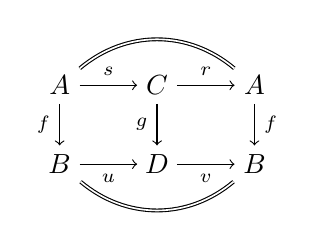
\begin{tikzpicture}[x=1.6em,y=1.5em]
  \node (At) at (0,1.3) {$A$};
  \node (C) at (2.2,1.3) {$C$};
  \node (Ar) at (4.4,1.3) {$A$};
  \node (B) at (0,-0.6) {$B$};
  \node (D) at (2.2,-0.6) {$D$};
  \node (Br) at (4.4,-0.6) {$B$};
  \draw[->] (0.45,1.3) -- (1.75,1.3) node[midway,above]{$\scriptstyle s$};
  \draw[->] (2.65,1.3) -- (3.95,1.3) node[midway,above]{$\scriptstyle r$};
  \draw[->] (0,0.85) -- (0,-0.15) node[midway,left]{$\scriptstyle f$};
  \draw[->] (2.2,0.85) -- (2.2,-0.15) node[midway,left]{$\scriptstyle g$};
  \draw[->] (4.4,0.85) -- (4.4,-0.15) node[midway,right]{$\scriptstyle f$};
  \draw[->] (0.45,-0.6) -- (1.75,-0.6) node[midway,below]{$\scriptstyle u$};
  \draw[->] (2.65,-0.6) -- (3.95,-0.6) node[midway,below]{$\scriptstyle v$};
  \draw[double] (At) to[out=40,in=140] (Ar);
  \draw[double] (B) to[out=-40,in=-140] (Br);
\end{tikzpicture}
\end{center}}

\begin{proposition}\label{prop:2-of-6-fibrant-objects}
设 $\mathcal{M}$ 是一个\trCategory，连同映射的两个类 $\rvW$ 与 $\rvF$，
使得：
\begin{itemize}
\item $\rvW$ 满足\trTwoOfThreeProperty，并且对\trRetract{}封闭。
\item $\rvF\cap\rvW$ 中一个映射的\trPullback{}仍在 $\rvF\cap\rvW$ 中，
  并且这些\trPullback{}总是存在。
\item $\rvW$ 中的每个映射都分解为某支 $\rvF\cap\rvW$ 中映射的\trSection{}%
  继以一支 $\rvF\cap\rvW$ 中的映射。
\end{itemize}
那么类 $\rvW$ 便满足\textbf{\trTwoOfSixProperty}：对任何可复合的三元组%
态射
\begin{center}
\begin{tikzpicture}[x=1.6em,y=1.5em]
  \node (A) at (0,0) {$A$};
  \node (B) at (2.2,1.4) {$B$};
  \node (D) at (4.4,0) {$D$};
  \node (C) at (2.2,-1.4) {$C$};
  \draw[->] (A) -- (B) node[pos=0.45,above,sloped]{$\scriptstyle f$};
  \draw[->] (B) -- (D) node[pos=0.45,above,sloped]{$\scriptstyle\overset{\sim}{hg}$};
  \draw[->] (A) -- (D) node[pos=0.5,above]{$\scriptstyle hgf$};
  \draw[->] (B) -- (C) node[pos=0.68,right]{$\scriptstyle g$};
  \draw[->] (A) -- (C) node[pos=0.6,below,sloped]{$\scriptstyle\overset{\sim}{gf}$};
  \draw[->] (C) -- (D) node[pos=0.5,below,sloped]{$\scriptstyle h$};
\end{tikzpicture}
\end{center}
若 $gf$ 与 $hg$ 属于类 $\rvW$，则 $f$、$g$、$h$ 与 $hgf$ 亦然。
\end{proposition}

\begin{proof}
对下方左侧所示的\trWeakEquivalence{} $hg$ 作分解，并作出 $p$ 沿 $h$ 的%
\trPullback{}与诱导映射 $t$：
\begin{center}
\begin{tikzpicture}[x=1.6em,y=1.5em]
  \node (Dp) at (2.6,1.3) {$D'$};
  \node (B) at (0,0) {$B$};
  \node (D) at (5.0,0) {$D$};
  \draw[->] (Dp) to[bend right=22] node[pos=0.5,above,sloped]{$\scriptstyle\overset{\sim}{r}$} (B);
  \draw[->] (B) to[bend right=18] node[pos=0.5,below,sloped]{$\scriptstyle\overset{\sim}{j}$} (Dp);
  \draw[double,->] (Dp) -- node[pos=0.5,above,sloped]{$\scriptstyle p$} (D);
  \draw[->] (B) -- (D) node[midway,below]{$\scriptstyle\overset{\sim}{hg}$};
\end{tikzpicture}
\qquad
\begin{tikzpicture}[x=1.6em,y=1.5em]
  \node (A) at (0,2.3) {$A$};
  \node (B) at (2.4,2.3) {$B$};
  \node (Cp) at (4.6,1.15) {$C'$};
  \node (Dp) at (6.4,1.15) {$D'$};
  \node (Br) at (8.8,1.15) {$B$};
  \node (C) at (3.8,-0.4) {$C$};
  \node (D) at (6.4,-0.4) {$D$};
  \draw[->] (A) -- (B) node[midway,above]{$\scriptstyle f$};
  \draw[dashed,->] (B) to[bend left=12] node[pos=0.55,above]{$\scriptstyle t$} (Cp);
  \draw[->] (B) to[bend left=18] node[pos=0.6,above,sloped]{$\scriptstyle\overset{\sim}{j}$} (Dp);
  \draw[->] (B) to[out=-95,in=45] node[pos=0.55,left]{$\scriptstyle g$} (C);
  \draw[->] (A) to[out=-80,in=160] node[pos=0.6,left]{$\scriptstyle\overset{\sim}{gf}$} (C);
  \draw[->] (Cp) -- (Dp) node[midway,above]{$\scriptstyle u$};
  \draw[->] (4.45,0.9) -- (4.45,0.05) node[midway,left]{$\scriptstyle q$};
  \node at (4.95,0.78) {$\scriptstyle\lrcorner$};
  \draw[->] (Dp) -- (Br) node[midway,above]{$\scriptstyle\overset{\sim}{r}$};
  \draw[double,->] (Dp) -- (D) node[midway,right]{$\scriptstyle p$};
  \draw[->] (C) -- (D) node[midway,below]{$\scriptstyle h$};
  \draw[double] (B) to[out=28,in=140] (Br);
\end{tikzpicture}
\end{center}
由\trTrivialFibration{}的\trPullback{}稳定性，映射 $q$ 属于 $\rvW$，于是由%
\trTwoOfThreeProperty{}及 $gf$ 属于 $\rvW$ 的假设，复合 $tf\colon A\to C'$
必属于 $\rvW$。映射 $f$ 是这一复合的一个\trRetract
\begin{center}
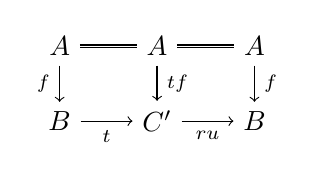
\begin{tikzpicture}[x=1.6em,y=1.5em]
  \node (A1) at (0,1.2) {$A$};
  \node (A2) at (2.2,1.2) {$A$};
  \node (A3) at (4.4,1.2) {$A$};
  \node (B) at (0,-0.6) {$B$};
  \node (Cp) at (2.2,-0.6) {$C'$};
  \node (B2) at (4.4,-0.6) {$B$};
  \draw[double] (A1) -- (A2);
  \draw[double] (A2) -- (A3);
  \draw[->] (A1) -- (B) node[midway,left]{$\scriptstyle f$};
  \draw[->] (A2) -- (Cp) node[midway,right]{$\scriptstyle tf$};
  \draw[->] (A3) -- (B2) node[midway,right]{$\scriptstyle f$};
  \draw[->] (B) -- (Cp) node[midway,below]{$\scriptstyle t$};
  \draw[->] (Cp) -- (B2) node[midway,below]{$\scriptstyle ru$};
\end{tikzpicture}
\end{center}
于是由类 $\rvW$ 的\trRetract{}封闭性，$f$ 属于 $\rvW$。现在由%
\trTwoOfThreeProperty{}即可进一步得出 $g$、$h$ 与 $hgf$ 都居于 $\rvW$ 中。
\end{proof}

\begin{corollary}\label{cor:2-of-6}
一个\trInfinityCosmos{}中的诸\trEquivalence{}满足\trTwoOfSixProperty。
\end{corollary}

\begin{proof}
只剩下论证\cref{prop:2-of-6-fibrant-objects} 的前提对任何\trInfinityCosmos{}%
中\trEquivalence{}、\trIsofibration{}与\trTrivialFibration{}的诸类成立。
第 1 章中的\cref{lem:equivalence-retracts-2-of-3} 证明：\trInfinityCosmos{}%
中的诸\trEquivalence{}还对\trRetract{}封闭并具有\trTwoOfThreeProperty。
第 1 章中的\cref{lem:trivial-fibration-stability} 证明：\trTrivialFibration{}%
类在\trPullback{}下稳定，而这些\trPullback{}在任何\trInfinityCosmos{}中都
存在。第 1 章中的\cref{lem:brown-factorization} 构造了所需的分解，由%
\trTwoOfThreeProperty，它把一个\trEquivalence{}分解为一支\trTrivialFibration{}%
的\trSection{}继以一支\trTrivialFibration。现在\cref{prop:2-of-6-fibrant-objects}
便适用于证明：任何\trInfinityCosmos{}中的诸\trEquivalence{}满足更强的%
\trTwoOfSixProperty。
\end{proof}

下述\cref{lem:brown-factorization-cfo} 的推论，传统上称作「Ken Brown 引理」，是证明%
\trCategoryOfFibrantObjects{}中种种\trLimit{}构造在\trPointwise{}\trWeakEquivalence{}之下
的不变性的关键所在。

\begin{lemma}[Ken Brown 引理]\label{lem:ken-brown}
考虑一个\trFunctor{} $F\colon\mathcal{M}\to\mathcal{N}$：其定义域是一个%
\trCategoryOfFibrantObjects，其陪域是一个配有满足\trTwoOfThreeProperty{}的
「\trWeakEquivalence」子范畴的\trCategory。若 $F$ 把\trTrivialFibration{}载为%
\trWeakEquivalence，则 $F$ 把 $\mathcal{M}$ 中的\trWeakEquivalence{}载为
$\mathcal{N}$ 中的\trWeakEquivalence。
\end{lemma}

\begin{proof}
由\cref{lem:brown-factorization-cfo}，\trCategoryOfFibrantObjects{}中的任何%
\trWeakEquivalence{}都可以分解为一支\trTrivialFibration{}的\trSection{}继以
一支\trTrivialFibration。
\begin{center}
\begin{tikzpicture}[x=1.6em,y=1.6em]
  \node (Pf) at (0.6,1.5) {$Pf$};
  \node (A) at (-1.4,0) {$A$};
  \node (B) at (3.0,0) {$B$};
  \draw[double,->] (Pf) to[bend right=28] node[pos=0.55,above,sloped]{$\scriptstyle\overset{\sim}{q}$} (A);
  \draw[->] (A) to[bend right=22] node[pos=0.5,below,sloped]{$\scriptstyle s$} (Pf);
  \draw[double,->] (Pf) -- node[pos=0.45,above,sloped]{$\scriptstyle p$} (B);
  \draw[->] (A) -- node[below]{$\scriptstyle\overset{\sim}{f}$} (B);
\end{tikzpicture}
\end{center}
由假设，映射 $q$ 与 $p$ 在 $F$ 之下的像是\trWeakEquivalence。由 $\mathcal{N}$
中\trWeakEquivalence{}的\trTwoOfThreeProperty，即可得出：$s$ 的像、从而
也有 $f$ 的像，都是\trWeakEquivalence。
\end{proof}

本节其余部分致力于\cref{lem:ken-brown} 的种种应用，以确立\trCategoryOfFibrantObjects{}%
中诸\trLimit{}的\trWeakEquivalence{}不变性。

\begin{lemma}\label{lem:pullback-we-between-fibrations}
在\trCategoryOfFibrantObjects{}中，诸\trFibration{}之间的一个\trWeakEquivalence{}拉回为
诸\trFibration{}之间的一个\trWeakEquivalence：
\begin{center}
\begin{tikzpicture}[x=1.6em,y=1.5em]
  \node (P) at (0,2) {$P$};
  \node (E) at (3.2,2) {$E$};
  \node (Q) at (1.2,1) {$Q$};
  \node (F) at (3.6,1) {$F$};
  \node (A) at (0,0) {$A$};
  \node (B) at (2.8,0) {$B$};
  \draw[->] (P) -- (E);
  \draw[->] (0.4,1.75) -- (1.05,1.28) node[pos=0.4,right]{$\scriptstyle u$};
  \node at (0.5,1.62) {$\scriptstyle\lrcorner$};
  \draw[->] (Q) -- (F);
  \draw[->] (0,1.7) -- (0,0.3) node[midway,left]{$\scriptstyle r$};
  \draw[->] (1.05,0.75) -- (0.4,0.26) node[pos=0.55,below]{$\scriptstyle s$};
  \node at (1.7,0.62) {$\scriptstyle\lrcorner$};
  \draw[double,->] (3.2,1.7) -- (3.2,0.3) node[midway,left]{$\scriptstyle p$};
  \draw[double,->] (3.75,0.7) -- (3.05,0.06) node[pos=0.6,right]{$\scriptstyle q$};
  \draw[->] (2.75,1.85) -- (3.35,1.28) node[pos=0.5,right]{$\scriptstyle\overset{\sim}{e}$};
  \draw[->] (0.55,0) -- (2.25,0) node[midway,below]{$\scriptstyle\overset{\sim}{f}$};
\end{tikzpicture}
\end{center}
\end{lemma}

\begin{proof}
由\cref{cor:slice-fibrant-objects}，\trCategoryOfFibrantObjects{} $\mathcal{M}$ 的诸切片
定义\trCategoryOfFibrantObjects，而且沿 $f$ 的\trPullback{}定义了一个\trFunctor{}
$f^{\ast}\colon\mathcal{M}_{/B}\to\mathcal{M}_{/A}$。注意所示\trDiagram{}中的映射
$u$ 是映射 $e$ 的\trPullback，于是由\cref{def:category-of-fibrant-objects}
的公理 (iii) 直接可得：拉回保持\trTrivialFibration。于是\cref{lem:ken-brown}
蕴含：它也保持诸\trEquivalence。
\end{proof}

类似脉络的其他结果则需要些许更为精致的论证。下面给出的证明原本归于
Reedy 的一部未出版手稿 \cite{bib99}，这部手稿隐含地孕育了我们在 C.4 节中
引入的「Reedy 范畴」概念。

\begin{proposition}\label{prop:pullback-map-fibration}
考虑\trCategoryOfFibrantObjects{}中的一个\trDiagram：
\begin{center}
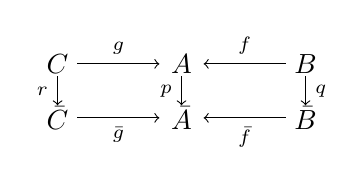
\begin{tikzpicture}[x=1.6em,y=1.5em]
  \node (C) at (0,1.3) {$C$};
  \node (A) at (2.8,1.3) {$A$};
  \node (B) at (5.6,1.3) {$B$};
  \node (Cb) at (0,0) {$\bar{C}$};
  \node (Ab) at (2.8,0) {$\bar{A}$};
  \node (Bb) at (5.6,0) {$\bar{B}$};
  \draw[->] (0.45,1.3) -- (2.3,1.3) node[midway,above]{$\scriptstyle g$};
  \draw[->] (5.15,1.3) -- (3.3,1.3) node[midway,above]{$\scriptstyle f$};
  \draw[->] (0,1.0) -- (0,0.3) node[midway,left]{$\scriptstyle r$};
  \draw[->] (2.8,1.0) -- (2.8,0.3) node[midway,left]{$\scriptstyle p$};
  \draw[->] (5.6,1.0) -- (5.6,0.3) node[midway,right]{$\scriptstyle q$};
  \draw[->] (0.45,0) -- (2.3,0) node[midway,below]{$\scriptstyle\bar{g}$};
  \draw[->] (5.15,0) -- (3.3,0) node[midway,below]{$\scriptstyle\bar{f}$};
\end{tikzpicture}
\end{center}
若映射 $r$ 与映射 $z\colon B\to A\times_{\bar{A}}\bar{B}$ 都是\trFibration{}或
都是\trTrivialFibration，那么从 $f$ 沿 $g$ 的\trPullback{}到 $\bar{f}$ 沿
$\bar{g}$ 的\trPullback{}的诱导映射，相应地仍是\trFibration{}或%
\trTrivialFibration。
\end{proposition}

\begin{proof}
由\trPullback{}的复合与消去，诱导映射 $t$ 分解为 $z$ 的一个\trPullback{}继以 $r$
的一个\trPullback，如下面所示
\begin{center}
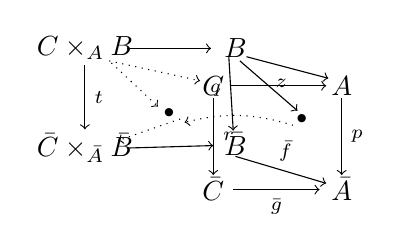
\begin{tikzpicture}[x=1.6em,y=1.5em]
  \node (CB) at (0,2.4) {$C\times_A B$};
  \node (B) at (3.4,2.4) {$B$};
  \node (A) at (5.8,1.5) {$A$};
  \node (C) at (2.9,1.5) {$C$};
  \node (d1) at (1.9,0.85) {$\scriptstyle\bullet$};
  \node (d2) at (4.9,0.7) {$\scriptstyle\bullet$};
  \node (CBb) at (0,0) {$\bar{C}\times_{\bar{A}}\bar{B}$};
  \node (Bb) at (3.4,0.1) {$\bar{B}$};
  \node (Cb) at (2.9,-1.0) {$\bar{C}$};
  \node (Ab) at (5.8,-1.0) {$\bar{A}$};
  \draw[->] (0.95,2.4) -- (2.85,2.4);
  \draw[dotted,->] (0.55,2.1) -- (2.6,1.62);
  \draw[dotted,->] (0.6,2.05) -- (1.65,1.0);
  \draw[->] (0,2.0) -- (0,0.45) node[midway,right]{$\scriptstyle t$};
  \draw[->] (3.65,2.2) -- (5.5,1.68);
  \draw[->] (3.3,1.5) -- (5.45,1.5);
  \draw[->] (3.5,2.1) -- (4.8,0.9) node[pos=0.45,right]{$\scriptstyle z$};
  \draw[->] (3.25,2.2) -- (3.35,0.42) node[pos=0.45,left]{$\scriptstyle q$};
  \draw[->] (2.9,1.2) -- (2.9,-0.65) node[midway,right]{$\scriptstyle r$};
  \draw[->] (5.8,1.2) -- (5.8,-0.65) node[midway,right]{$\scriptstyle p$};
  \node at (2.2,0.6) {$\scriptstyle\lrcorner$};
  \node at (5.2,0.45) {$\scriptstyle\lrcorner$};
  \draw[dotted,->] (2.15,0.7) -- (0.75,0.18);
  \draw[dotted,->] (4.7,0.55) to[bend right=15] (2.25,0.62);
  \draw[->] (0.95,0) -- (2.9,0.06);
  \draw[->] (3.4,-0.2) -- (5.45,-0.85) node[pos=0.55,above]{$\scriptstyle\bar{f}$};
  \draw[->] (3.35,-1.0) -- (5.3,-1.0) node[midway,below]{$\scriptstyle\bar{g}$};
\end{tikzpicture}
\end{center}
于是当这两支映射都是\trFibration{}或都是\trTrivialFibration{}时，它亦然。
\end{proof}

类似地，我们有如下结果，其对偶形式有时称作「\textbf{粘合引理}」
（gluing lemma）。

\begin{proposition}\label{prop:pullback-map-equivalence}
在一个\trCategoryOfFibrantObjects{}中，如下形式之\trDiagram{}的两个水平行各自的%
\trPullback{}之间的诱导映射仍是一个\trWeakEquivalence：
\begin{center}
\begin{tikzpicture}[x=1.6em,y=1.5em]
  \node (C) at (0,1.3) {$C$};
  \node (A) at (2.8,1.3) {$A$};
  \node (B) at (5.6,1.3) {$B$};
  \node (Cb) at (0,0) {$\bar{C}$};
  \node (Ab) at (2.8,0) {$\bar{A}$};
  \node (Bb) at (5.6,0) {$\bar{B}$};
  \draw[->] (0.45,1.3) -- (2.3,1.3) node[midway,above]{$\scriptstyle g$};
  \draw[->] (5.15,1.3) -- (3.3,1.3) node[midway,above]{$\scriptstyle f$};
  \draw[->] (0,1.0) -- (0,0.3) node[midway,left]{$\scriptstyle\overset{\sim}{r}$};
  \draw[->] (2.8,1.0) -- (2.8,0.3) node[midway,left]{$\scriptstyle\overset{\sim}{p}$};
  \draw[->] (5.6,1.0) -- (5.6,0.3) node[midway,right]{$\scriptstyle\overset{\sim}{q}$};
  \draw[->] (0.45,0) -- (2.3,0) node[midway,below]{$\scriptstyle\bar{g}$};
  \draw[->] (5.15,0) -- (3.3,0) node[midway,below]{$\scriptstyle\bar{f}$};
\end{tikzpicture}
\end{center}
\end{proposition}

第 3 章中的\cref{prop:pullback-invariance} 的证明同样适用于任何%
\trRightProper{}\trCategoryOfFibrantObjects，但正如我们将发现的，\trRightProperness{}%
这一假设实际上并不必要。

\begin{proof}
由\cref{ex:cospan-cfo}，对任何\trCategoryOfFibrantObjects{} $\mathcal{M}$ 都存在一个%
\trCategoryOfFibrantObjects{} $\mathcal{M}^{\perp}$，其
\begin{itemize}
\item 对象是\trCospan{} $C\xrightarrow{g}A\xleftarrow{f}B$，其中右腿是
  $\mathcal{M}$ 中的一支\trFibration；
\item \trWeakEquivalence{}是\trPointwise{}\trWeakEquivalence；并且
\item \trFibration{}是形如下图的\trDiagram，其中映射 $r$、$p$ 与 $q$
  都是\trFibration，而诱导映射 $z\colon B\to A\times_{\bar{A}}\bar{B}$
  亦然：
\begin{center}
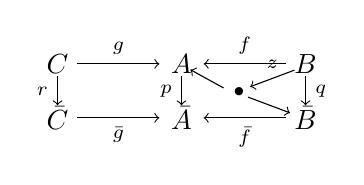
\begin{tikzpicture}[x=1.6em,y=1.5em]
  \node (C) at (0,1.3) {$C$};
  \node (A) at (2.8,1.3) {$A$};
  \node (B) at (5.6,1.3) {$B$};
  \node (Cb) at (0,0) {$\bar{C}$};
  \node (Ab) at (2.8,0) {$\bar{A}$};
  \node (Bb) at (5.6,0) {$\bar{B}$};
  \node (dot) at (4.1,0.62) {$\scriptstyle\bullet$};
  \draw[->] (0.45,1.3) -- (2.3,1.3) node[midway,above]{$\scriptstyle g$};
  \draw[->] (5.15,1.3) -- (3.3,1.3) node[midway,above]{$\scriptstyle f$};
  \draw[->] (0,1.0) -- (0,0.3) node[midway,left]{$\scriptstyle r$};
  \draw[->] (2.8,1.0) -- (2.8,0.3) node[midway,left]{$\scriptstyle p$};
  \draw[->] (5.6,1.0) -- (5.6,0.3) node[midway,right]{$\scriptstyle q$};
  \draw[->] (0.45,0) -- (2.3,0) node[midway,below]{$\scriptstyle\bar{g}$};
  \draw[->] (5.15,0) -- (3.3,0) node[midway,below]{$\scriptstyle\bar{f}$};
  \draw[->] (5.35,1.15) -- (4.35,0.75) node[pos=0.5,above]{$\scriptstyle z$};
  \draw[->] (3.75,0.72) -- (3.0,1.16);
  \draw[->] (4.3,0.5) -- (5.25,0.12);
  \node at (4.42,0.5) {$\scriptstyle\lrcorner$};
\end{tikzpicture}
\end{center}
\end{itemize}
而所需的诸\trLimit{}则逐点继承自 $\mathcal{M}$。由%
\cref{prop:pullback-map-fibration}，拉回\trFunctor{}
$\lim\colon\mathcal{M}^{\perp}\to\mathcal{M}$ 把\trTrivialFibration{}载为%
\trTrivialFibration，于是由\cref{lem:ken-brown}，它也保持诸%
\trWeakEquivalence。
\end{proof}

\begin{corollary}\label{cor:finite-products}
在一个\trCategoryOfFibrantObjects{}中，诸\trFibration{}、诸\trTrivialFibration{}或诸%
\trWeakEquivalence{}的有限\trProduct{}仍是\trFibration{}、%
\trTrivialFibration{}或\trWeakEquivalence。
\end{corollary}

\begin{proof}
一族有限多个映射 $\{f_i\colon A_i\to\bar{A}_i\}_{i=1,\dots,n}$ 的\trProduct{}%
可以归纳地构造为\trTerminal{}对象 $1$ 上的一个\trPullback：
\begin{center}
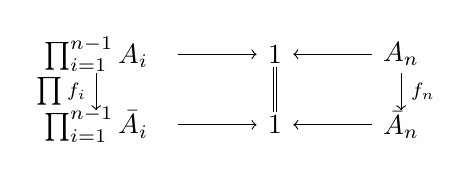
\begin{tikzpicture}[x=1.9em,y=1.5em]
  \node (P1) at (0,1.3) {$\prod\nolimits_{i=1}^{n-1}A_i$};
  \node (1t) at (3.4,1.3) {$1$};
  \node (An) at (5.8,1.3) {$A_n$};
  \node (P2) at (0,-0.4) {$\prod\nolimits_{i=1}^{n-1}\bar{A}_i$};
  \node (1b) at (3.4,-0.4) {$1$};
  \node (Anb) at (5.8,-0.4) {$\bar{A}_n$};
  \draw[->] (1.55,1.3) -- (3.05,1.3);
  \draw[->] (5.25,1.3) -- (3.75,1.3);
  \draw[->] (0,0.85) -- (0,-0.05) node[midway,left]{$\scriptstyle\prod f_i$};
  \draw[double] (3.4,1.0) -- (3.4,-0.1);
  \draw[->] (5.8,0.85) -- (5.8,-0.05) node[midway,right]{$\scriptstyle f_n$};
  \draw[->] (1.55,-0.4) -- (3.05,-0.4);
  \draw[->] (5.25,-0.4) -- (3.75,-0.4);
\end{tikzpicture}
\end{center}
当每个映射 $f_i$ 都是\trFibration{}或\trTrivialFibration{}时，由%
\cref{prop:pullback-map-fibration}及从二元\trProduct{}情形起步的归纳，
这些映射的\trProduct{}亦然。当每个映射 $f_i$ 都是\trWeakEquivalence{}时，
同样的结论由\cref{prop:pullback-map-equivalence} 得出。
\end{proof}

类似地，诸\trFibration{}之塔的诸\trLimit{}在\trPointwise{}%
\trWeakEquivalence{}下不变：

\begin{proposition}\label{prop:tower-limits}
考虑\trCategoryOfFibrantObjects{}中诸可数\trFibration{}塔之间的一个\trNaturalTransformation
\begin{center}
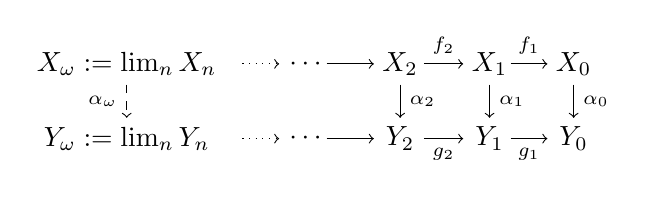
\begin{tikzpicture}[x=1.9em,y=1.5em]
  \node (Xw) at (0,1.3) {$X_\omega:=\lim_n X_n$};
  \node (Xd) at (3.4,1.3) {$\cdots$};
  \node (X2) at (5.2,1.3) {$X_2$};
  \node (X1) at (6.9,1.3) {$X_1$};
  \node (X0) at (8.5,1.3) {$X_0$};
  \node (Yw) at (0,-0.5) {$Y_\omega:=\lim_n Y_n$};
  \node (Yd) at (3.4,-0.5) {$\cdots$};
  \node (Y2) at (5.2,-0.5) {$Y_2$};
  \node (Y1) at (6.9,-0.5) {$Y_1$};
  \node (Y0) at (8.5,-0.5) {$Y_0$};
  \draw[dotted,->] (2.2,1.3) -- (2.9,1.3);
  \draw[->] (3.8,1.3) -- (4.7,1.3);
  \draw[->] (5.65,1.3) -- (6.4,1.3) node[midway,above]{$\scriptstyle f_2$};
  \draw[->] (7.3,1.3) -- (8.0,1.3) node[midway,above]{$\scriptstyle f_1$};
  \draw[dotted,->] (2.2,-0.5) -- (2.9,-0.5);
  \draw[->] (3.8,-0.5) -- (4.7,-0.5);
  \draw[->] (5.65,-0.5) -- (6.4,-0.5) node[midway,below]{$\scriptstyle g_2$};
  \draw[->] (7.3,-0.5) -- (8.0,-0.5) node[midway,below]{$\scriptstyle g_1$};
  \draw[dashed,->] (0,0.8) -- (0,-0.0) node[midway,left]{$\scriptstyle\alpha_\omega$};
  \draw[->] (5.2,0.8) -- (5.2,0.0) node[midway,right]{$\scriptstyle\alpha_2$};
  \draw[->] (6.9,0.8) -- (6.9,0.0) node[midway,right]{$\scriptstyle\alpha_1$};
  \draw[->] (8.5,0.8) -- (8.5,0.0) node[midway,right]{$\scriptstyle\alpha_0$};
\end{tikzpicture}
\end{center}
\begin{enumerate}[label=(\roman*)]
\item 若对每个 $n\geq 0$，映射
  $\langle\alpha_n,f_n\rangle\colon X_n\to Y_n\times_{Y_{n-1}}X_{n-1}$
  是\trFibration{}或\trTrivialFibration，\footnote{为使 $n=0$ 的情形有
  意义，约定 $X_{-1}$ 与 $Y_{-1}$ 为\trTerminal{}对象，于是此时所考虑的
  映射即 $\alpha_0$。}那么诸\trLimit{}之间的诱导映射 $\alpha_\omega$
  亦然。
\item 若对每个 $n\geq 0$，映射 $\alpha_n$ 是\trWeakEquivalence，那么诸%
  \trLimit{}之间的诱导映射 $\alpha_\omega$ 亦然。
\end{enumerate}
\end{proposition}

\begin{proof}
当 (i) 的假设在\trCategoryOfFibrantObjects{} $\mathcal{M}$ 中成立时，诸\trFibration{}塔之
诸\trLimit{}之间的诱导映射 $\alpha_\omega\colon X_\omega\to Y_\omega$
本身就是下述\trFibration{}塔或\trTrivialFibration{}塔的一个极限复合
\begin{center}
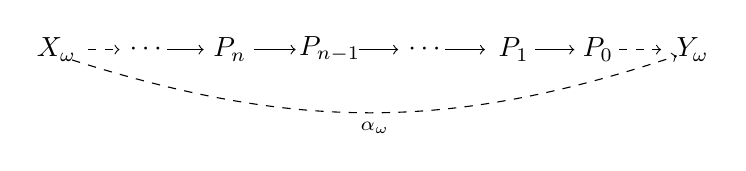
\begin{tikzpicture}[x=1.9em,y=1.5em]
  \node (Xw) at (0,0) {$X_\omega$};
  \node (D1) at (1.7,0) {$\cdots$};
  \node (Pn) at (3.3,0) {$P_n$};
  \node (Pn1) at (5.2,0) {$P_{n-1}$};
  \node (D2) at (7.0,0) {$\cdots$};
  \node (P1) at (8.7,0) {$P_1$};
  \node (P0) at (10.3,0) {$P_0$};
  \node (Yw) at (12.1,0) {$Y_\omega$};
  \draw[dashed,->] (0.6,0) -- (1.2,0);
  \draw[->] (2.1,0) -- (2.8,0);
  \draw[->] (3.75,0) -- (4.55,0);
  \draw[->] (5.75,0) -- (6.5,0);
  \draw[->] (7.4,0) -- (8.15,0);
  \draw[->] (9.1,0) -- (9.85,0);
  \draw[dashed,->] (10.7,0) -- (11.5,0);
  \draw[dashed,->] (0.3,-0.25) to[bend right=18] node[pos=0.5,below]{$\scriptstyle\alpha_\omega$} (11.8,-0.15);
\end{tikzpicture}
\end{center}
其中每一层都是下述映射的一个\trPullback，而该映射被假设为\trFibration{}或%
\trTrivialFibration：
\begin{center}
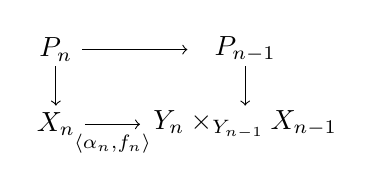
\begin{tikzpicture}[x=1.9em,y=1.5em]
  \node (Pn) at (0,1.2) {$P_n$};
  \node (Pn1) at (3.6,1.2) {$P_{n-1}$};
  \node (Xn) at (0,-0.6) {$X_n$};
  \node (YX) at (3.6,-0.6) {$Y_n\times_{Y_{n-1}}X_{n-1}$};
  \draw[->] (0.5,1.2) -- (2.5,1.2);
  \node at (0.55,0.9) {$\scriptstyle\lrcorner$};
  \draw[->] (0,0.8) -- (0,-0.15);
  \draw[->] (3.6,0.8) -- (3.6,-0.15);
  \draw[->] (0.55,-0.6) -- (1.6,-0.6) node[midway,below]{$\scriptstyle\langle\alpha_n,f_n\rangle$};
\end{tikzpicture}
\end{center}
从底部开始，$P_0$ 定义为 $\alpha_0$ 沿 $Y_\omega$ 的\trLimit{}\trCone{}%
的一条腿的\trPullback：
\begin{center}
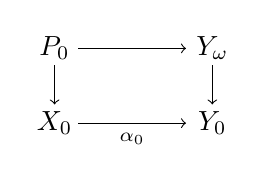
\begin{tikzpicture}[x=1.9em,y=1.5em]
  \node (P0) at (0,1.2) {$P_0$};
  \node (Yw) at (3.0,1.2) {$Y_\omega$};
  \node (X0) at (0,-0.6) {$X_0$};
  \node (Y0) at (3.0,-0.6) {$Y_0$};
  \draw[->] (0.45,1.2) -- (2.5,1.2);
  \node at (0.55,0.9) {$\scriptstyle\lrcorner$};
  \draw[->] (0,0.8) -- (0,-0.15);
  \draw[->] (3.0,0.8) -- (3.0,-0.15);
  \draw[->] (0.45,-0.6) -- (2.5,-0.6) node[midway,below]{$\scriptstyle\alpha_0$};
\end{tikzpicture}
\end{center}
由构造，$P_0$ 容许一个到\trPullback{} $Y_1\times_{Y_0}X_0$ 的\trCanonical{}%
映射，而 $P_1$ 被定义为如下\trPullback：
\begin{center}
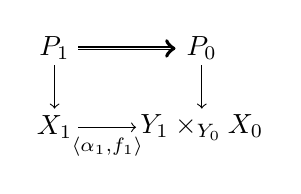
\begin{tikzpicture}[x=1.9em,y=1.5em]
  \node (P1) at (0,1.2) {$P_1$};
  \node (P0) at (2.8,1.2) {$P_0$};
  \node (X1) at (0,-0.7) {$X_1$};
  \node (YX) at (2.8,-0.7) {$Y_1\times_{Y_0}X_0$};
  \draw[double,->] (0.45,1.2) -- (2.3,1.2);
  \node at (0.55,0.9) {$\scriptstyle\lrcorner$};
  \draw[->] (0,0.8) -- (0,-0.25);
  \draw[->] (2.8,0.8) -- (2.8,-0.25);
  \draw[->] (0.45,-0.7) -- (1.55,-0.7) node[midway,below]{$\scriptstyle\langle\alpha_1,f_1\rangle$};
\end{tikzpicture}
\end{center}
继续归纳地做下去，诸\trFibration{}的塔
$P_n\rvFarrow P_{n-1}$ 的\trLimit{}可以被看出与 $\omega^{\mathrm{op}}\times 2$
形状的\trDiagram{}之\trLimit{}相重合，该\trDiagram{}由映射 $f_n$、$g_n$ 与 $\alpha_n$
构成。由于此\trDiagram{}顶行的包含
$\omega^{\mathrm{op}}\hookrightarrow\omega^{\mathrm{op}}\times 2$
是始的，这个\trLimit{}复原出 $X_\omega$，而诸\trFibration{}之塔的复合
复原出映射 $\alpha_\omega$。于是，由\cref{def:category-of-fibrant-objects}
的公理 (iii) 与 (iv)，诱导映射 $\alpha_\omega$ 相应地仍是\trFibration{}或%
\trTrivialFibration。

第二个陈述现在这样得出：把\cref{lem:ken-brown} 用于\trLimit{}\trFunctor{}
$\lim\colon\mathcal{M}^{\omega^{\mathrm{op}}}\to\mathcal{M}$，其定义域是诸%
\trFibration{}塔的\trCategory{}（见\cref{ex:towers-cfo}）。
\end{proof}

在这个证明中，我们再一次利用了这样一个事实：取值于\trCategoryOfFibrantObjects{}的%
\trDiagram{}\trCategory{}自身也可以配备\trCategoryOfFibrantObjects{}的结构——至少对某些
类型的\trDiagram{}与某些\trDiagram{}形状是如此。我们现在对一个格外有用的%
\trDiagram{}族——即以\textbf{逆范畴}（inverse categories）为标的%
\trDiagram{}——更系统地确立这一结果。

\begin{definition}\label{def:inverse-category}
一个\trCategory{} $\mathcal{J}$ 是一个\textbf{逆范畴}（inverse category），
若存在一个\trFunctor{} $\mathrm{deg}\colon\mathcal{J}\to\omega^{\mathrm{op}}$
使其反映恒同。\footnote{若把 $\omega$ 换成\trOrdinalCategory，数学内容并无
实质性改变。我们限制于有限度数的原因在于：\cref{def:category-of-fibrant-objects}
只要求 $\omega^{\mathrm{op}}$ 标引的塔之\trLimit{}（见\cref{prop:general-towers}(i)）。}
\end{definition}

度函子给 $\mathcal{J}$ 的每个对象指派一个自然数度数，使得一切非恒同态射
都「降低度数」——也就是说，其定义域对象的度数严格大于其陪域对象的
度数。度函子之于逆范畴的用处在于：它使我们得以归纳地指定以度数有界之
对象的诸全子范畴
\begin{center}
\begin{tikzpicture}[x=2.1em,y=1.4em]
  \node (J0) at (0,0) {$\mathcal{J}_{\leq 0}$};
  \node (D1) at (1.8,0) {$\cdots$};
  \node (Jn1) at (3.7,0) {$\mathcal{J}_{\leq n-1}$};
  \node (Jn) at (6.0,0) {$\mathcal{J}_{\leq n}$};
  \node (D2) at (7.8,0) {$\cdots$};
  \node (Jc) at (10.4,0) {$\operatorname{colim}_{n\in\omega}\mathcal{J}_{\leq n}\cong\mathcal{J}$};
  \draw[right hook->] (0.7,0) -- (1.35,0);
  \draw[right hook->] (2.25,0) -- (3.1,0);
  \draw[right hook->] (4.4,0) -- (5.35,0);
  \draw[right hook->] (6.65,0) -- (7.35,0);
  \draw[right hook->] (8.25,0) -- (9.1,0);
\end{tikzpicture}
\end{center}
为标的\trDiagram，从而定义一个 $\mathcal{J}$ 标引的\trDiagram{}或%
\trNaturalTransformation{}的数据。要把 $X\in\mathcal{M}^{\mathcal{J}_{\leq n-1}}$ 扩张为
$\mathcal{M}^{\mathcal{J}_{\leq n}}$ 中的一个\trDiagram，需要对每个度数为 $n$ 的
对象 $i$ 指定一个对象 $X^i\in\mathcal{M}$，连同
一支从 $X^i$ 指向如下\trLimit{}的映射 $X^i\to\partial^i X$：
\begin{rveq}\label{eq:boundary-object}
\partial^i X:=\operatorname{lim}_{i\to j}X_j
:=\operatorname{lim}\Big(\;
\underset{\textstyle i\ne j}{\mathcal{J}_{\leq n-1}}
\xrightarrow{\ \mathrm{cod}\ }
\mathcal{J}_{\leq n-1}
\xrightarrow{\ X\ }
\mathcal{M}\;\Big)
\end{rveq}
其以 $\mathcal{J}$ 中的非恒同映射 $i\to j$ 为标引。

\begin{observation}[边界数据作为一个\trWeightedLimit]\label{obs:boundary-weighted-limit}
正如记号所提示的那样，对象 $\partial^i X$ 应当被理解为与 $X^i$ 相关联的
「\trBoundary{}数据」之对象。这一直觉可以经由\trWeightedLimit{}的形式理论
而变得精确，这即便在非富集的语境中也例示了它们的用处。

回顾附录 A 中的\cref{def:weighted-limit-colimit-axiomatic}(i)：\trDiagram
$X\in\mathcal{M}^{\mathcal{J}}$ 在对象 $i\in\mathcal{J}$ 处被可表示函子
$\mathcal{J}(i,-)\in\mathcal{S}et^{\mathcal{J}}$ 加权的\trLimit{}即对象
$X^i$。把可表示函子的\textbf{\trBoundary}
$\partial\mathcal{J}(i,-)\in\mathcal{S}et^{\mathcal{J}}$ 定义为由下式给出的函子
\[
\partial\mathcal{J}(i,j):=\begin{cases}
\mathcal{J}(i,j) & \deg(j)<\deg(i)\\
\varnothing & \deg(j)\geq\deg(i)
\end{cases}
\]
将\eqref{eq:boundary-object} 与附录 A 中的%
\cref{rem:unenriched-indexing-categories} 的公式相比较，我们观察到
$\operatorname{lim}_{\partial\mathcal{J}(i,-)}X\cong\partial^i X$。

回顾附录 A 中的\cref{def:weighted-limit-colimit-axiomatic}：\trWeightedLimit{}%
对权是反变函子性的。于是，自然包含
$\partial\mathcal{J}(i,-)\hookrightarrow\mathcal{J}(i,-)$ 便诱导出一个%
\trCanonical{}映射
\[
X^i\cong\operatorname{lim}_{\mathcal{J}(i,-)}X
\xrightarrow{\ m^i\ }
\operatorname{lim}_{\partial\mathcal{J}(i,-)}X
\cong\partial^i X
\]
介于诸\trWeightedLimit{}之间。提前借用 C.4 节中\cref{def:latching-matching-objects}的术语，我们把
$\partial^i X$ 称作\trDiagram{} $X$ 的第 $i$ 个\textbf{匹配对象}，并把
$m^i\colon X^i\to\partial^i X$ 称作第 $i$ 个\textbf{匹配映射}。
\end{observation}

出于稍后便会明朗的原因，我们定义：

\begin{definition}\label{def:fibrant-diagram}
设 $\mathcal{M}$ 是一个\trCategoryOfFibrantObjects，并设 $\mathcal{J}$ 是一个逆范畴。
\begin{itemize}
\item 一个\textbf{纤维性图表}（fibrant diagram）是一个\trDiagram
  $X\in\mathcal{M}^{\mathcal{J}}$，它具有如下性质：对每个
  $i\in\mathcal{J}$，匹配映射 $m^i\colon X^i\to\partial^i X$
  是一个\trFibration。
\item 一个\textbf{纤维性自然变换}（fibrant natural transformation）是
  纤维性图表之间的一个\trNaturalTransformation{}
  $\alpha\colon X\to Y\in\mathcal{M}^{\mathcal{J}}$，使得对每个
  $i\in\mathcal{J}$，由诸匹配映射构成的方块中的\trPullback{}所定义的
  \textbf{相对匹配映射}（relative matching map）$\hat{m}^i$ 是一个%
  \trFibration：
\begin{rveq}\label{eq:relative-matching-map}
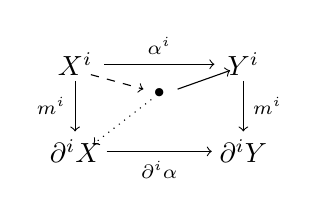
\begin{tikzpicture}[x=1.9em,y=1.5em]
  \node (Xi) at (0,1.2) {$X^i$};
  \node (Yi) at (3.2,1.2) {$Y^i$};
  \node (dot) at (1.6,0.5) {$\scriptstyle\bullet$};
  \node (dX) at (0,-0.9) {$\partial^i X$};
  \node (dY) at (3.2,-0.9) {$\partial^i Y$};
  \draw[->] (0.55,1.2) -- (2.65,1.2) node[midway,above]{$\scriptstyle\alpha^i$};
  \draw[dashed,->] (0.3,0.95) -- (1.3,0.6);
  \draw[->] (1.95,0.6) -- (2.95,1.05);
  \draw[dotted,->] (1.45,0.35) -- (0.35,-0.72);
  \node at (1.92,0.32) {$\scriptstyle\lrcorner$};
  \draw[->] (0,0.8) -- (0,-0.42) node[midway,left]{$\scriptstyle m^i$};
  \draw[->] (3.2,0.8) -- (3.2,-0.42) node[midway,right]{$\scriptstyle m^i$};
  \draw[->] (0.6,-0.9) -- (2.6,-0.9) node[midway,below]{$\scriptstyle\partial^i\alpha$};
\end{tikzpicture}
\end{rveq}
\end{itemize}
\end{definition}

例如，形状为 $\omega$ 的纤维性图表即是一个\trFibration{}塔，正如%
\cref{prop:tower-limits} 中那样。该结果第一条陈述所提及的那些映射，恰是与
纤维性图表之间的\trNaturalTransformation{} $\alpha$ 相关联的诸相对匹配映射，
于是第一条假设恰好断言：$\alpha$ 是一个纤维性自然变换。下述\cref{prop:tower-limits}
的推广是第 6 章中的\cref{prop:flexible-weights-homotopical} 的非富集版本。

\begin{proposition}\label{prop:general-towers}
\begin{enumerate}[label=(\roman*)]
\item \trCategoryOfFibrantObjects{} $\mathcal{M}$ 容有任何一个以逆范畴 $\mathcal{J}$ 为
  标引的纤维性图表 $X\in\mathcal{M}^{\mathcal{J}}$ 的诸\trLimit{}，其中
  $\operatorname{lim}_{\mathcal{J}}X\in\mathcal{M}$%
  \yizhu{原书于此印作 $\operatorname{lim}_{\mathcal{J}}F$，疑为 $X$ 之误，
  此处径改。}被构造为如下一座塔%
  \footnote{这些对象是受限\trDiagram{}的诸\trLimit{}，下标指示标引范畴。}的%
  \trLimit{}
\[
\operatorname{lim}_{\mathcal{J}}X
:=\operatorname{lim}_{\omega^{\mathrm{op}}}
\Big(\cdots\to
\operatorname{lim}_{\mathcal{J}_{\leq n}}X\to
\operatorname{lim}_{\mathcal{J}_{\leq n-1}}X\to
\cdots\to
\operatorname{lim}_{\mathcal{J}_{\leq 0}}X\Big)
\]
其每一层都是一个\trPullback
\begin{center}
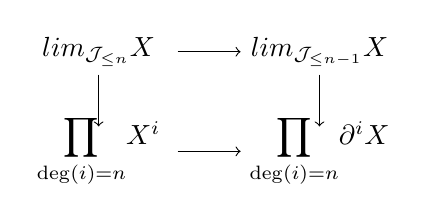
\begin{tikzpicture}[x=1.9em,y=1.5em]
  \node (Ln) at (0,1.3) {${\displaystyle\operatorname{lim}_{\mathcal{J}_{\leq n}}X}$};
  \node (Ln1) at (4.2,1.3) {${\displaystyle\operatorname{lim}_{\mathcal{J}_{\leq n-1}}X}$};
  \node (P1) at (0,-1.1) {${\displaystyle\prod_{\deg(i)=n}}X^i$};
  \node (P2) at (4.2,-1.1) {${\displaystyle\prod_{\deg(i)=n}}\partial^i X$};
  \draw[->] (1.5,1.3) -- (2.7,1.3);
  \node at (1.55,1.0) {$\scriptstyle\lrcorner$};
  \draw[->] (0,0.75) -- (0,-0.5);
  \draw[->] (4.2,0.75) -- (4.2,-0.5);
  \draw[->] (1.5,-1.1) -- (2.7,-1.1);
\end{tikzpicture}
\end{center}
特别地，\trLimit{}\trCone{} $\operatorname{lim}_{\mathcal{J}}X\to X^i$
的每条腿都是\trFibration，纤维性图表 $X$ 的像中的每个映射亦然。
\item 对纤维性图表之间的任何纤维性自然变换
  $\alpha\colon X\to Y\in\mathcal{M}^{\mathcal{J}}$，诱导映射
  $\operatorname{lim}_{\mathcal{J}}X\to\operatorname{lim}_{\mathcal{J}}Y$
  是一座塔的极限复合，其第 $n$ 层是映射 $p_n$ 的一个\trPullback，该映射
  构造为下图中的拉回：
\begin{rveq}\label{eq:tower-cube}
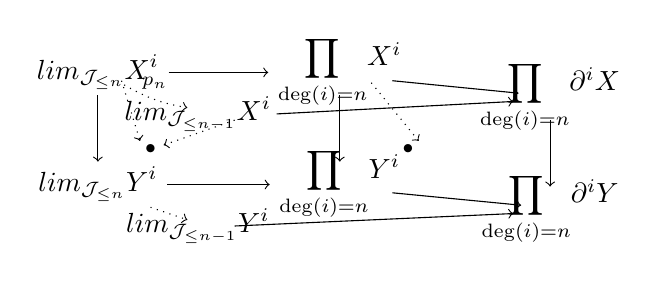
\begin{tikzpicture}[x=1.9em,y=1.5em]
  \node (An) at (0,2.6) {${\displaystyle\operatorname{lim}_{\mathcal{J}_{\leq n}}X^i}$};
  \node (Bn) at (4.6,2.6) {${\displaystyle\prod_{\deg(i)=n}}X^i$};
  \node (Cn) at (8.6,2.0) {${\displaystyle\prod_{\deg(i)=n}}\partial^i X$};
  \node (An1) at (1.9,1.6) {${\displaystyle\operatorname{lim}_{\mathcal{J}_{\leq n-1}}X^i}$};
  \node (d1) at (1.0,0.75) {$\scriptstyle\bullet$};
  \node (d2) at (5.9,0.75) {$\scriptstyle\bullet$};
  \node (F) at (0,-0.1) {${\displaystyle\operatorname{lim}_{\mathcal{J}_{\leq n}}Y^i}$};
  \node (G) at (4.6,-0.1) {${\displaystyle\prod_{\deg(i)=n}}Y^i$};
  \node (H) at (8.6,-0.7) {${\displaystyle\prod_{\deg(i)=n}}\partial^i Y$};
  \node (I) at (1.9,-1.1) {${\displaystyle\operatorname{lim}_{\mathcal{J}_{\leq n-1}}Y^i}$};
  \draw[->] (An) -- (Bn);
  \draw[->] (5.6,2.4) -- (8.0,2.1);
  \draw[dotted,->] (0.5,2.3) to[bend right=10] node[pos=0.5,above]{$\scriptstyle p_n$} (1.7,1.75);
  \draw[dotted,->] (0.45,2.4) -- (0.8,0.95);
  \draw[dotted,->] (2.6,1.45) -- (1.25,0.85);
  \draw[dotted,->] (5.2,2.35) -- (6.1,0.95);
  \draw[->] (3.4,1.6) -- (7.9,1.9);
  \node at (1.28,0.55) {$\scriptstyle\lrcorner$};
  \node at (6.18,0.55) {$\scriptstyle\lrcorner$};
  \draw[->] (0,2.05) -- (0,0.45);
  \draw[->] (4.6,2.05) -- (4.6,0.45);
  \draw[->] (8.6,1.45) -- (8.6,-0.15);
  \draw[->] (2.6,-1.1) -- (7.9,-0.8);
  \draw[->] (F) -- (G);
  \draw[->] (5.6,-0.3) -- (8.05,-0.6);
  \draw[dotted,->] (1.0,-0.65) -- (1.7,-0.95);
\end{tikzpicture}
\end{rveq}
此外，每个分量映射 $\alpha^i\colon X^i\rvFarrow Y^i$ 都是\trFibration。
\end{enumerate}
\end{proposition}

\begin{proof}
注意切片\trCategory{} $i\backslash\mathcal{J}_{n-1}$ 仍是一个逆范畴，其度\trFunctor{}为
\[
i\backslash\mathcal{J}_{n-1}\xrightarrow{\ \mathrm{cod}\ }\mathcal{J}_{n-1}
\xrightarrow{\ \deg\ }\omega^{\mathrm{op}}
\]
其中每个对象的度数至多为 $n-1$。在 $i$ 的度数为 $1$ 的情形，该\trCategory{}%
只有恒同箭头，于是由归纳法我们可以假定\eqref{eq:boundary-object} 所定义的
$\partial^i X$ 存在。现在，(i) 的结果由直接检视这一构造的\trUniversalProperty{}%
而得出，一如\cref{prop:tower-limits} 之证明中的做法。最后的论断由这一构造
随之而来，其验证留给\cref{ex:component-fibrations}。

由 (i) 可知，诸逆向极限之间的诱导映射定义为\trCategoryOfArrows{}
$\mathcal{M}^{\mathbf{2}}$ 中一个 $\omega^{\mathrm{op}}$ 标引\trDiagram{}的%
\trLimit{}：
\begin{center}
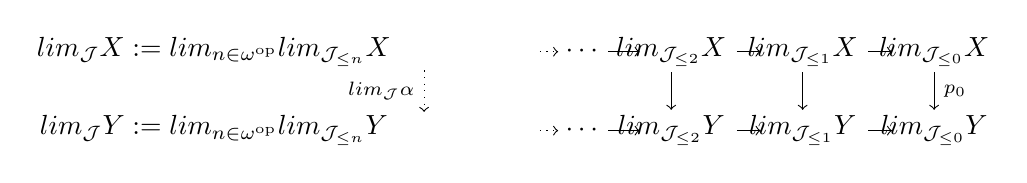
\begin{tikzpicture}[x=1.9em,y=1.5em]
  \node (Xt) at (0,1.3) {$\operatorname{lim}_{\mathcal{J}}X:=\operatorname{lim}_{n\in\omega^{\mathrm{op}}}\operatorname{lim}_{\mathcal{J}_{\leq n}}X$};
  \node (Xd) at (7.0,1.3) {$\cdots$};
  \node (X2) at (8.7,1.3) {$\operatorname{lim}_{\mathcal{J}_{\leq 2}}X$};
  \node (X1) at (11.2,1.3) {$\operatorname{lim}_{\mathcal{J}_{\leq 1}}X$};
  \node (X0) at (13.7,1.3) {$\operatorname{lim}_{\mathcal{J}_{\leq 0}}X$};
  \node (Yt) at (0,-0.6) {$\operatorname{lim}_{\mathcal{J}}Y:=\operatorname{lim}_{n\in\omega^{\mathrm{op}}}\operatorname{lim}_{\mathcal{J}_{\leq n}}Y$};
  \node (Yd) at (7.0,-0.6) {$\cdots$};
  \node (Y2) at (8.7,-0.6) {$\operatorname{lim}_{\mathcal{J}_{\leq 2}}Y$};
  \node (Y1) at (11.2,-0.6) {$\operatorname{lim}_{\mathcal{J}_{\leq 1}}Y$};
  \node (Y0) at (13.7,-0.6) {$\operatorname{lim}_{\mathcal{J}_{\leq 0}}Y$};
  \draw[dotted,->] (6.2,1.3) -- (6.55,1.3);
  \draw[->] (7.5,1.3) -- (8.1,1.3);
  \draw[->] (9.95,1.3) -- (10.4,1.3);
  \draw[->] (12.45,1.3) -- (12.9,1.3);
  \draw[dotted,->] (6.2,-0.6) -- (6.55,-0.6);
  \draw[->] (7.5,-0.6) -- (8.1,-0.6);
  \draw[->] (9.95,-0.6) -- (10.4,-0.6);
  \draw[->] (12.45,-0.6) -- (12.9,-0.6);
  \draw[dotted,->] (4.0,0.85) -- (4.0,-0.15) node[midway,left]{$\scriptstyle\operatorname{lim}_{\mathcal{J}}\alpha$};
  \draw[->] (8.7,0.8) -- (8.7,-0.1);
  \draw[->] (11.2,0.8) -- (11.2,-0.1);
  \draw[->] (13.7,0.8) -- (13.7,-0.1) node[midway,right]{$\scriptstyle p_0$};
\end{tikzpicture}
\end{center}
在 (ii) 的假设下，由\cref{prop:tower-limits}(i) 的证明可得：映射
$\operatorname{lim}_{\mathcal{J}}\alpha$ 随之分解为一座塔的极限复合，其
底层是映射 $p_0$ 沿上方较低水平复合的\trPullback，其下一层是出现于最右侧
方块中的映射 $p_1$ 的\trPullback，再下一层是出现于第二右侧方块中的映射
$p_2$ 的\trPullback，依此类推，其中在每个方块中，$p_n$ 都是从左上角到
右下余跨度之\trPullback{}的映射。映射 $p_0$ 是以度数为零的对象为标的诸
相对匹配映射之积，因而是一个\trFibration。在立方体 \eqref{eq:tower-cube}
中应用\trPullback{}的复合与消去可知：由 (i)，顶面与底面都是拉回方块，于是映射
$p_n$——从初始顶点到左面中的拉回——是从
$\prod_{\deg(i)=n}X^i$ 到右面中拉回的对应映射的一个\trPullback。这一映射是
以度数为 $n$ 的对象为标的诸相对匹配映射之积，从而是一个\trFibration，故
$p_n$ 也是一个\trFibration。于是，由\cref{prop:tower-limits}(i)，诱导映射
$\operatorname{lim}_{\mathcal{J}}\alpha\colon\operatorname{lim}_{\mathcal{J}}X\to\operatorname{lim}_{\mathcal{J}}Y$
也是一个\trFibration。这就证明了 (ii) 中除最后一个断言之外的全部内容，
而后者同样留给\cref{ex:component-fibrations}。
\end{proof}

我们还想进一步断言：对以逆范畴为标引的纤维性图表之间的任何%
\trPointwise{}\trWeakEquivalence{} $\alpha\colon X\to Y\in\mathcal{M}^{\mathcal{J}}$，
诱导映射 $\operatorname{lim}_{\mathcal{J}}X\to\operatorname{lim}_{\mathcal{J}}Y$
是一个\trWeakEquivalence。一如\cref{prop:tower-limits}(ii) 的证明，这需要
一个具有独立兴趣的中间结果，它与练习 6.1.iii 密切相关。

\begin{proposition}\label{prop:fibrant-diagram-cfo}
设 $\mathcal{M}$ 是一个配有\trFibration{}类 $\rvF$ 与\trWeakEquivalence{}%
类 $\rvW$ 的\trCategoryOfFibrantObjects，并设 $\mathcal{J}$ 是一个逆范畴。由纤维性图表
与其间的全部\trNaturalTransformation{}构成的\trCategory{}
$\mathcal{M}^{\mathcal{J}}$ 继承一个\trCategoryOfFibrantObjects{}的结构，其中：
\begin{itemize}
\item 诸\trWeakEquivalence{}是诸分量居于 $\rvW$ 中的那些%
  \trNaturalTransformation{}；
\item 诸\trFibration{}是诸纤维性自然变换，即那些
  $\alpha\colon X\to Y\in\mathcal{M}^{\mathcal{J}}$，使得对每个
  $i\in\mathcal{J}$，相对匹配映射
  $X^i\xrightarrow{\ \hat{m}^i\ \rvFarrow\ }Y^i\times_{\partial^i Y}\partial^i X$
  属于 $\rvF$；
\item 诸\trTrivialFibration{}是那些
  $\alpha\colon X\to Y\in\mathcal{M}^{\mathcal{J}}$，使得对每个
  $i\in\mathcal{J}$，相对匹配映射
  $X^i\xrightarrow{\ \hat{m}^i\ \rvTFarrow\ }Y^i\times_{\partial^i Y}\partial^i X$
  属于 $\rvF\cap\rvW$。
\end{itemize}
\end{proposition}

\begin{proof}
这一证明对读者而言是一项颇为冗长的练习，它只是把 C.4 节中的相应论证特化到
这一「单边」情形。使用一个略有不同的公理化的类似结果的证明，可见
\cite[9.2.4]{bib94}。
\end{proof}

这一切工作的回报是如下结果。

\begin{proposition}\label{prop:inverse-limits-we}
设 $\mathcal{M}$ 是一个\trCategoryOfFibrantObjects，并设 $\mathcal{J}$ 是一个逆范畴。
那么，对纤维性图表之间的任何\trPointwise{}\trWeakEquivalence{}
$\alpha\colon X\to Y\in\mathcal{M}^{\mathcal{J}}$，诸\trLimit{}之间的诱导
映射 $\operatorname{lim}_{\mathcal{J}}X\to\operatorname{lim}_{\mathcal{J}}Y$
是一个\trWeakEquivalence。
\end{proposition}

\begin{proof}
我们利用\cref{prop:fibrant-diagram-cfo}，它赋予纤维性图表的\trCategory{}
$\mathcal{M}^{\mathcal{J}}$ 以\trCategoryOfFibrantObjects{}的结构。考虑 $\rvF$ 中或
$\rvF\cap\rvW$ 中的一个映射 $\alpha\colon X\to Y\in\mathcal{M}^{\mathcal{J}}$。
由\cref{prop:general-towers}(ii)，这一映射是一座映射塔的极限复合，其每一层
都是我们已假设居于 $\rvF$ 或 $\rvF\cap\rvW$ 中的那些映射之积的一个%
\trPullback。由于类 $\rvF$ 与 $\rvF\cap\rvW$ 对\trProduct、\trPullback{}与
塔的\trLimit{}封闭，现在已然清楚：\trLimit{}\trFunctor{}保持这些类。而它也
保持类 $\rvW$ 这一事实，则由\cref{lem:ken-brown} 得出。
\end{proof}

\begin{exercise}\label{ex:cospan-cfo}
证明：对任何\trCategoryOfFibrantObjects{} $\mathcal{M}$，都存在一个%
\trCategoryOfFibrantObjects{} $\mathcal{M}^{\perp}$，其
\begin{itemize}
\item 对象是\trCospan{} $C\xrightarrow{g}A\xleftarrow{f}B$，其中右腿是
  $\mathcal{M}$ 中的一支\trFibration；
\item \trWeakEquivalence{}是\trPointwise{}\trWeakEquivalence；并且
\item \trFibration{}是形如下图的\trDiagram，其中映射 $r$、$p$ 与 $q$ 都是%
  \trFibration，而诱导映射 $z\colon B\to A\times_{\bar{A}}\bar{B}$ 亦然：
\begin{center}
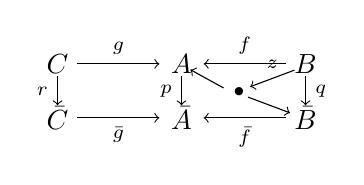
\begin{tikzpicture}[x=1.6em,y=1.5em]
  \node (C) at (0,1.3) {$C$};
  \node (A) at (2.8,1.3) {$A$};
  \node (B) at (5.6,1.3) {$B$};
  \node (Cb) at (0,0) {$\bar{C}$};
  \node (Ab) at (2.8,0) {$\bar{A}$};
  \node (Bb) at (5.6,0) {$\bar{B}$};
  \node (dot) at (4.1,0.62) {$\scriptstyle\bullet$};
  \draw[->] (0.45,1.3) -- (2.3,1.3) node[midway,above]{$\scriptstyle g$};
  \draw[->] (5.15,1.3) -- (3.3,1.3) node[midway,above]{$\scriptstyle f$};
  \draw[->] (0,1.0) -- (0,0.3) node[midway,left]{$\scriptstyle r$};
  \draw[->] (2.8,1.0) -- (2.8,0.3) node[midway,left]{$\scriptstyle p$};
  \draw[->] (5.6,1.0) -- (5.6,0.3) node[midway,right]{$\scriptstyle q$};
  \draw[->] (0.45,0) -- (2.3,0) node[midway,below]{$\scriptstyle\bar{g}$};
  \draw[->] (5.15,0) -- (3.3,0) node[midway,below]{$\scriptstyle\bar{f}$};
  \draw[->] (5.35,1.15) -- (4.35,0.75) node[pos=0.5,above]{$\scriptstyle z$};
  \draw[->] (3.75,0.72) -- (3.0,1.16);
  \draw[->] (4.3,0.5) -- (5.25,0.12);
  \node at (4.42,0.5) {$\scriptstyle\lrcorner$};
\end{tikzpicture}
\end{center}
\end{itemize}
而所需的诸\trLimit{}则逐点继承自 $\mathcal{M}$。
\end{exercise}

\begin{exercise}\label{ex:towers-cfo}
将\cref{prop:fibrant-diagram-cfo} 特化，以描述\trCategoryOfFibrantObjects{} $\mathcal{M}$
中诸\trFibration{}塔的\trCategory{} $\mathcal{M}^{\omega^{\mathrm{op}}}$
上的\trCategoryOfFibrantObjects{}结构，并以之为\cref{prop:tower-limits}(ii) 的证明补全
收官。
\end{exercise}

\begin{exercise}\label{ex:component-fibrations}
\cref{prop:reedy-components}
\begin{enumerate}[label=(\roman*)]
\item 验证\cref{prop:general-towers}(i) 中所构造的\trLimit{}\trCone{}的
  每条腿都是一个\trFibration。
\item 由此推论：纤维性图表的像中的每个态射都是一个\trFibration。
\item 沿同样的路线论证，验证纤维性自然变换的每个分量都是一个%
  \trFibration。
\end{enumerate}
\end{exercise}

\begin{exercise}\label{ex:prove-c123}
证明\cref{prop:fibrant-diagram-cfo}，并判定\cref{ex:cospan-cfo} 与%
\cref{ex:towers-cfo} 是否为这一结果的特例。
\end{exercise}
